\documentclass{article}

\usepackage{Sweave}
\begin{document}
\Sconcordance{concordance:accuracy.tex:accuracy.Rnw:%
1 2 1 1 0 35 1 1 21 3 0 1 1 9 0 1 12 2 0 1 1 10 0 1 4 3 1 1 6 1 3 2 1 1 %
6 1 3 2 1}


\title{Accuracy}

\author{Mc}
\maketitle
\section*{Introduction}
In plots we recast the results of simulations in terms of accuracy. We compute the accuracy of each method (continous or categorical), for each level of \(\rho\) (see below) by computing the  the following quantities:
\begin{itemize}
  \item false positive (FP)  runs with  with a significant test under a true null hypothesis
  \item true positive (TP) runs with a significant test under a false null-hypothesis 
  \item true negative (TN) runs  with a nonsignificant result under a true null-hypothesis
  \item false negative (FN) runs with a nonsignificant result under a false null-hypothesis

\end{itemize}

\section*{Setup}
\subsection*{Model}
Two continuous latent variables (\(\eta\) and \(\xi\) ) are created with N cases, sharing a correlation equal to \(\rho\). A measure \(x\) of \(\xi\) is created with reliability \(rel\), and then  is dichotomized accordingly to \(p\) \(1-p\) into \(c\). The correlations \( r_pe=r(\eta,x) \)  and \( r_pb=r(\eta,c) \) are computed, their p-value and significance (at .05) is recorded.
\subsection*{Design}
\(\rho=(0,.1,.2,.3,.4,.5,.6,.7) \)
\(rel=(0.3, 0.4 ,0.5, 0.6, 0.7 ,0.8 0.9) \) 


\subsection*{Computation of quantities}

\begin{itemize}
  \item Continuous false positive (FP\_C)  freq of runs with continuous test p.<.05 and \(\rho\)=0  
  \item Continuous true positive (TP\_C)  freq of runs with continuous test p.<.05 and \(\rho\)>0
  \item Continuous true negative (TN\_C)  freq of runs  with continuous test p.>=.05 and \(\rho\)=0
  \item false negative (FN\_C)  freq of runs  with continuous test p.>=.05 and \(\rho\)>0
\end{itemize}

The same quantities are computed for the categorical indicator (*\_S).

\begin{Schunk}
\begin{Soutput}
Accuracy for continuous indicator
\end{Soutput}
\begin{Soutput}
  rho    SENS_C    SPEC_C
1 0.1 0.1050000 0.9507143
2 0.2 0.2511429 0.9507143
3 0.3 0.4511429 0.9507143
4 0.4 0.6090000 0.9507143
5 0.5 0.7204286 0.9507143
6 0.6 0.7974286 0.9507143
7 0.7 0.8618571 0.9507143
\end{Soutput}
\begin{Soutput}
Accuracy for categorical indicator
\end{Soutput}
\begin{Soutput}
  rho     SENS_S    SPEC_S
1 0.1 0.08414286 0.9498571
2 0.2 0.17957143 0.9498571
3 0.3 0.33785714 0.9498571
4 0.4 0.47128571 0.9498571
5 0.5 0.61057143 0.9498571
6 0.6 0.70114286 0.9498571
7 0.7 0.77900000 0.9498571
\end{Soutput}
\end{Schunk}


\subsubsection*{Figure 1: Sensitivity of the two methods}

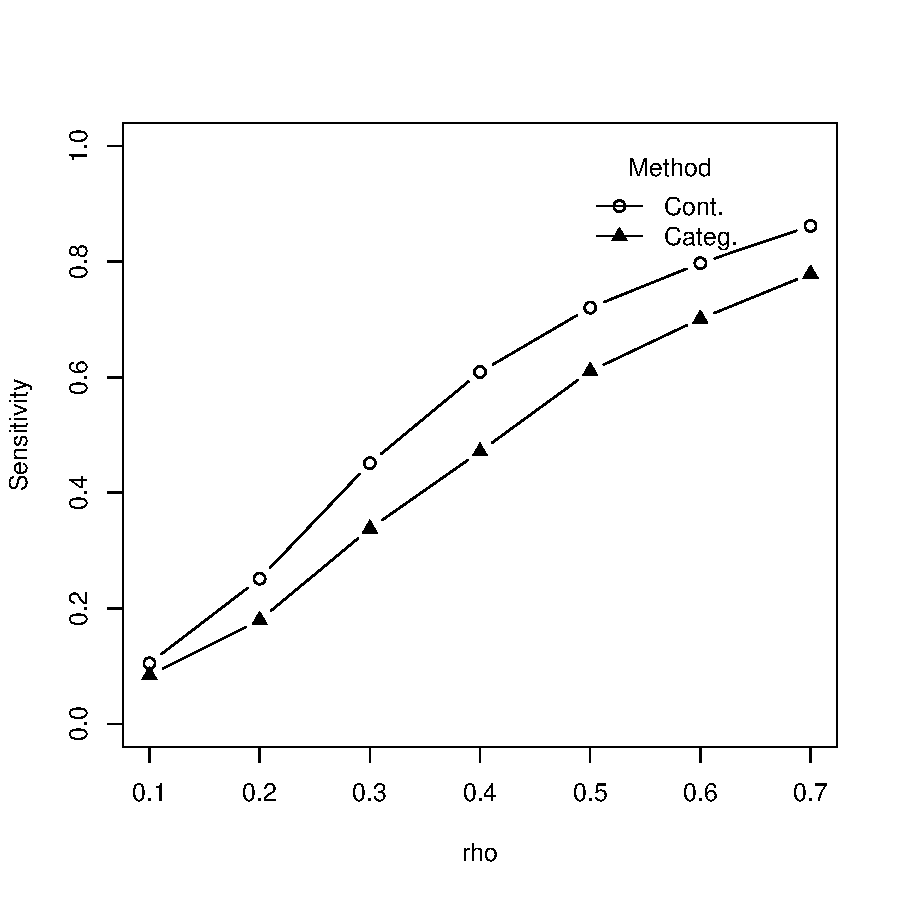
\includegraphics{accuracy-dd}

\subsubsection*{Figure 1: Specificity of the two methods}

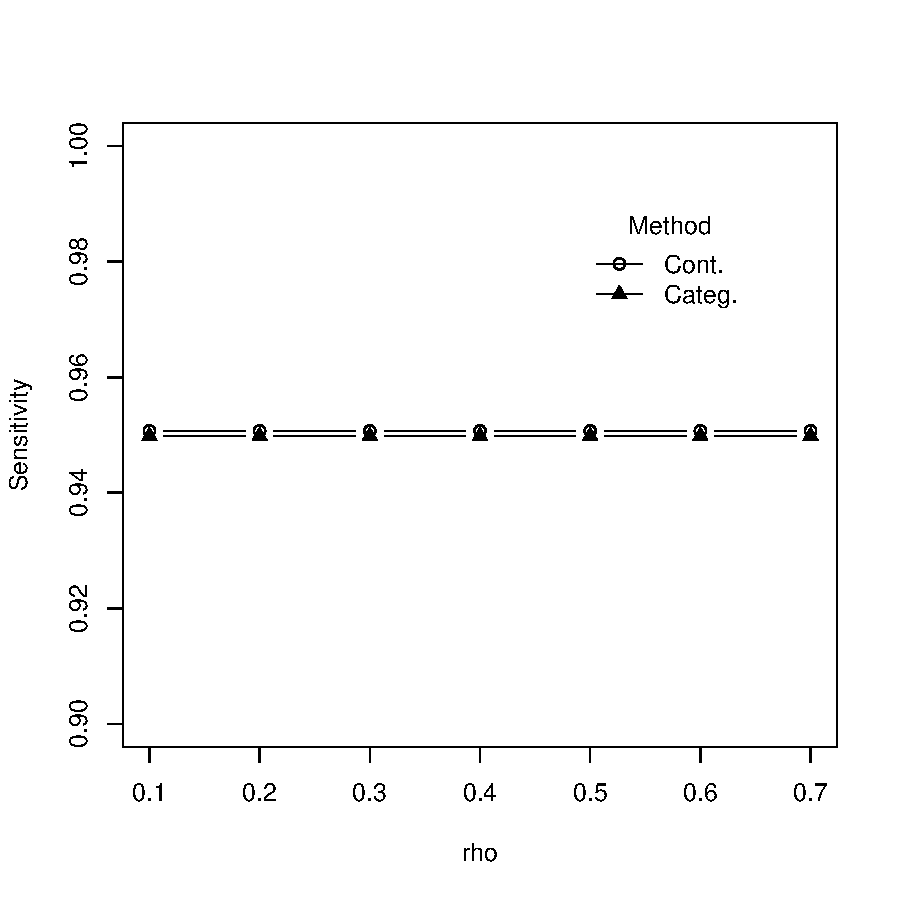
\includegraphics{accuracy-ee}


\end{document}
